%%%%%%%%%%%%%%%%%%%%%%%%%%%%%%%%%%%%%
%                                   %
% Compile with XeLaTeX and biber    %
%                                   %
% Questions or comments:            %
%                                   %
% joshua dot mcneill at uga dot edu %
%                                   %
%%%%%%%%%%%%%%%%%%%%%%%%%%%%%%%%%%%%%

\documentclass{beamer}
  % Read in standard preamble (cosmetic stuff)
  %%%%%%%%%%%%%%%%%%%%%%%%%%%%%%%%%%%%%%%%%%%%%%%%%%%%%%%%%%%%%%%%
% This is a standard preamble used in for all slide documents. %
% It basically contains cosmetic settings.                     %
%                                                              %
% Joshua McNeill                                               %
% joshua dot mcneill at uga dot edu                            %
%%%%%%%%%%%%%%%%%%%%%%%%%%%%%%%%%%%%%%%%%%%%%%%%%%%%%%%%%%%%%%%%

% Beamer settings
% \usetheme{Berkeley}
\usetheme{CambridgeUS}
% \usecolortheme{dove}
% \usecolortheme{rose}
\usecolortheme{seagull}
\usefonttheme{professionalfonts}
\usefonttheme{serif}
\setbeamertemplate{bibliography item}{}

% Packages and settings
\usepackage{fontspec}
  \setmainfont{Charis SIL}
\usepackage{hyperref}
  \hypersetup{colorlinks=true,
              allcolors=blue}
\usepackage{graphicx}
  \graphicspath{{../../figures/}}
\usepackage[normalem]{ulem}
\usepackage{enumerate}

% Document information
\author{M. McNeill}
\title[FREN2001]{Français 2001}
\institute{\url{joshua.mcneill@uga.edu}}
\date{}

%% Custom commands
% Lexical items
\newcommand{\lexi}[1]{\textit{#1}}
% Gloss
\newcommand{\gloss}[1]{`#1'}
\newcommand{\tinygloss}[1]{{\tiny`#1'}}
% Orthographic representations
\newcommand{\orth}[1]{$\langle$#1$\rangle$}
% Utterances (pragmatics)
\newcommand{\uttr}[1]{`#1'}
% Sentences (pragmatics)
\newcommand{\sent}[1]{\textit{#1}}
% Base dir for definitions
\newcommand{\defs}{../definitions}


  % Packages and settings

  % Document information
  \subtitle[Verbes (\lexi{acheter} et \lexi{appeler})]{Les verbes comme \lexi{acheter} et \lexi{appeler}}

\begin{document}
  % Read in the standard intro slides (title page and table of contents)
  \begin{frame}
    \titlepage
    \tiny{Office: % Basically a variable for office hours location
Gilbert 121\\
          Office hours: % Basically a variable for office hours
 lundi, mercredi, vendredi 10:10--11:10
}
  \end{frame}

  \begin{frame}{Annonces}
    \begin{itemize}
      \item L'atelier de discussion vendredi
      \item[] \tinygloss{Conversation workshop Friday}
      \item L'activité sur la nourriture lundi
      \item[] \tinygloss{Food activity Monday}
    \end{itemize}
  \end{frame}

  \begin{frame}{Les verbes comme \lexi{acheter}}
    \begin{center}
      \begin{tabular}{l | l l | l l}
  \multicolumn{5}{c}{acheter \gloss{to buy}} \\
      & \multicolumn{2}{l |}{singulier} & \multicolumn{2}{l}{pluriel} \\
  \hline
  1re & j'         & achète             & nous        & achetons \\
  2e  & tu         & achètes            & vous        & achetez \\
  \hline
  3e  & il (masc)  &                    & ils (masc)  & \\
      & elle (fem) & achète             & elles (fem) & achètent \\
      & on         &                    &             & \\
\end{tabular}

    \end{center}
  \end{frame}

  \begin{frame}{Les verbes comme \lexi{appeler}}
    \begin{center}
      \begin{tabular}{l | l l | l l}
  \multicolumn{5}{c}{appeler \gloss{to call}} \\
      & \multicolumn{2}{l |}{singulier} & \multicolumn{2}{l}{pluriel} \\
  \hline
  1re & j'         & appelle            & nous        & appelons \\
  2e  & tu         & appelles           & vous        & appelez \\
  \hline
  3e  & il (masc)  &                    & ils (masc)  & \\
      & elle (fem) & appelle            & elles (fem) & appellent \\
      & on         &                    &             & \\
\end{tabular}

    \end{center}
    L'important, c'est que le \orth{e} est prononcé /ɛ/ pour les deux types de verbes\\
    \tinygloss{The important thing is that the \orth{e} is pronounced /ɛ/ for both types of verbs}
  \end{frame}

  \begin{frame}{Acheter pour manger est appelé}
    % Si nous achetons les aliments suivants, comment nous appelons le repas résultant? \\
    % \tinygloss{If we buy the following foods, what do we call the resulting meal?}
    \begin{columns}
      \column{0.5\textwidth}
        \scriptsize
        \begin{enumerate}
          \item Nous achetons \underline{\uncover<2->{des yaourts et des fruits}},
          \item et nous appelons ce repas \underline{\uncover<3->{le petit-déjeuner}}.
          \item<4-> Nous achetons \underline{\uncover<5->{du pain au chocolat et du jus de pomme}},
          \item<4-> et nous appelons ce repas \underline{\uncover<6->{le petit-déjeuner}}.
          \item<7-> Nous achetons \underline{\uncover<8->{un poisson et du riz}},
          \item<7-> et nous appelons ce repas \underline{\uncover<9->{le dîner}}.
          \item<10-> Nous achetons \underline{\uncover<11->{un sandwich et de la soupe}},
          \item<10-> et nous appelons ce repas \underline{\uncover<12->{le déjeuner}}.
          \item<13-> Nous achetons \underline{\uncover<14->{un poulet et des pommes de terre}},
          \item<13-> et nous appelons ce repas \underline{\uncover<15->{le dîner}}.
        \end{enumerate}
      \column{0.5\textwidth}
        \begin{minipage}[c][0.6\textheight]{\linewidth}
          \begin{center}
            \only<-3>{
              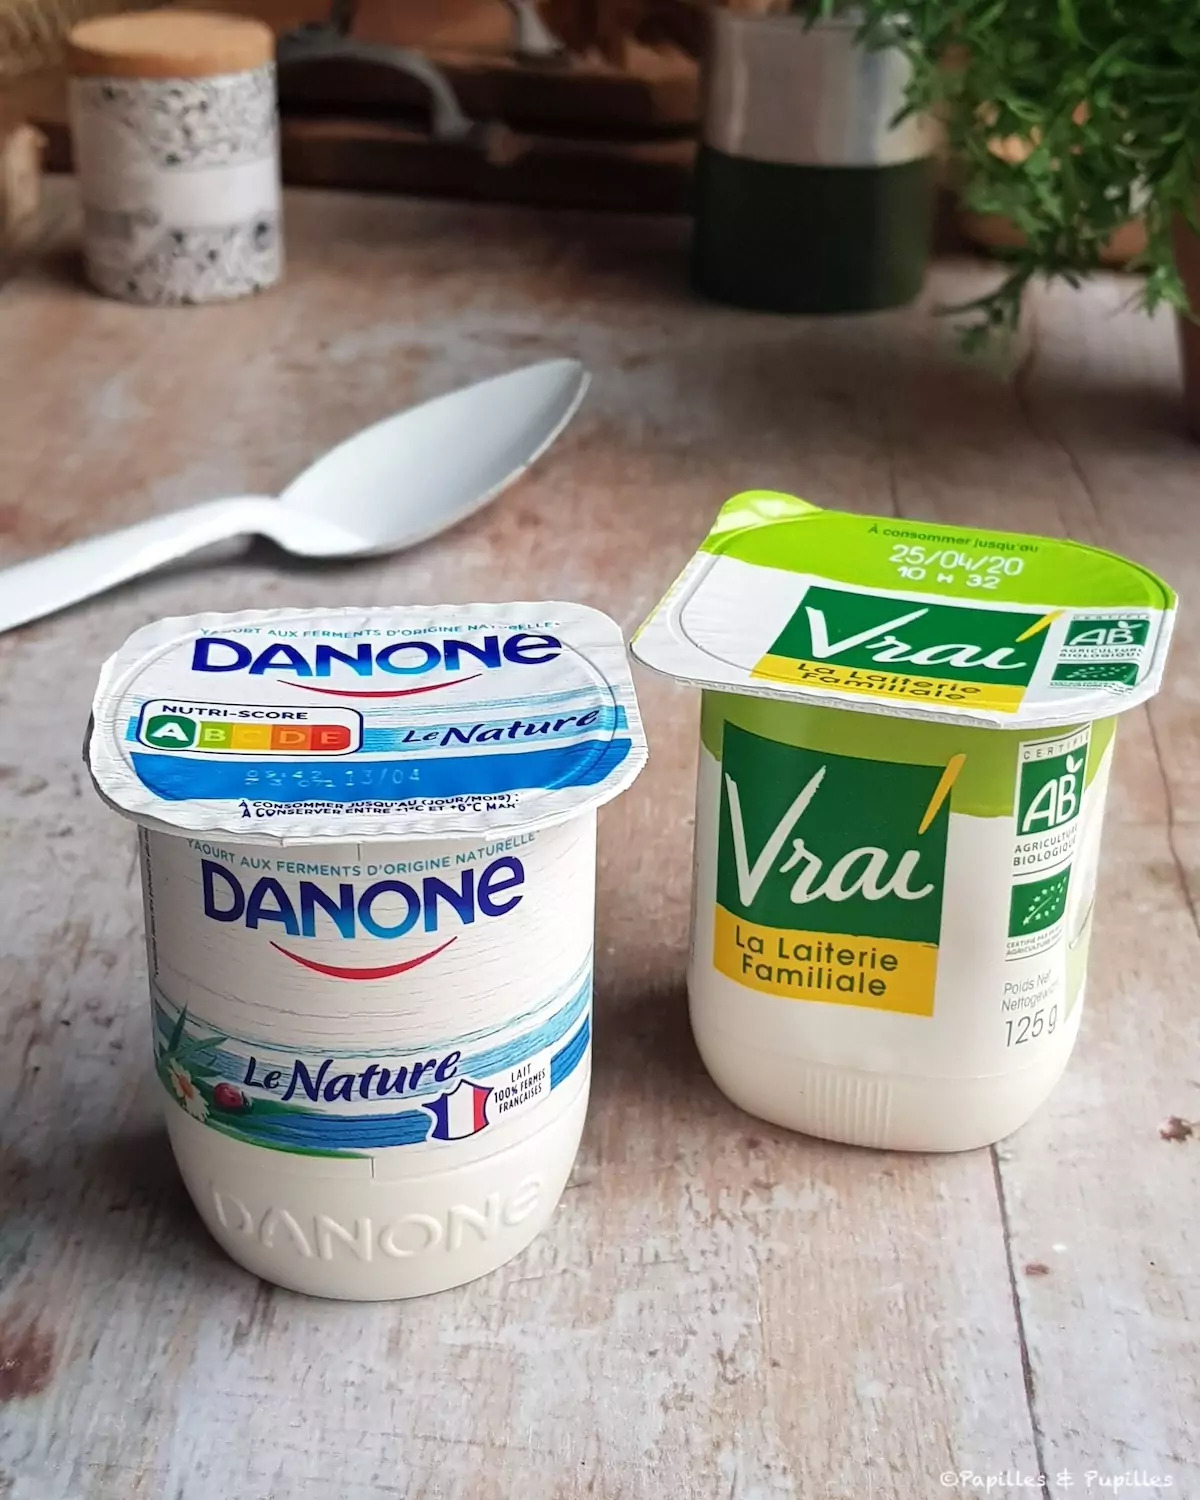
\includegraphics[scale=0.07]{yaourts.jpg} \\
              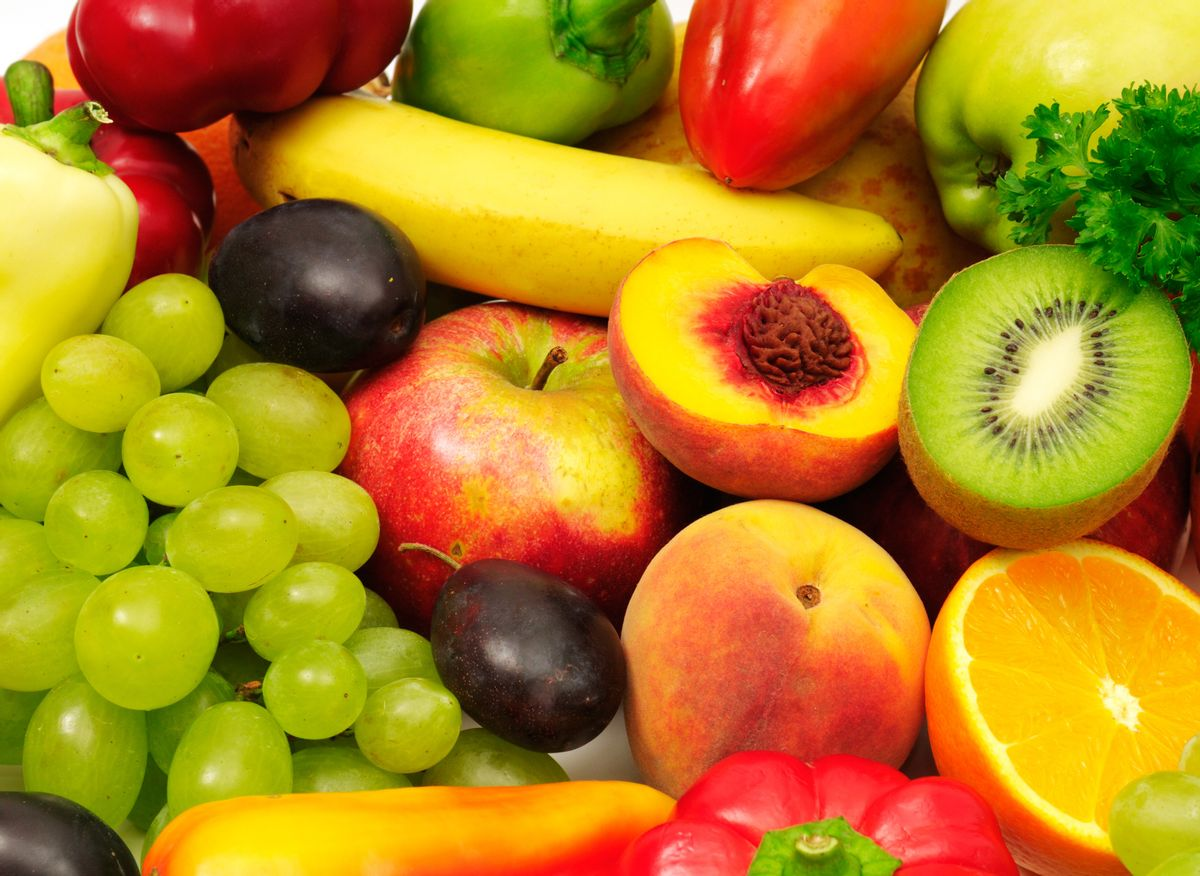
\includegraphics[scale=0.1]{fruits.jpg}
            }
            \only<4-6>{
              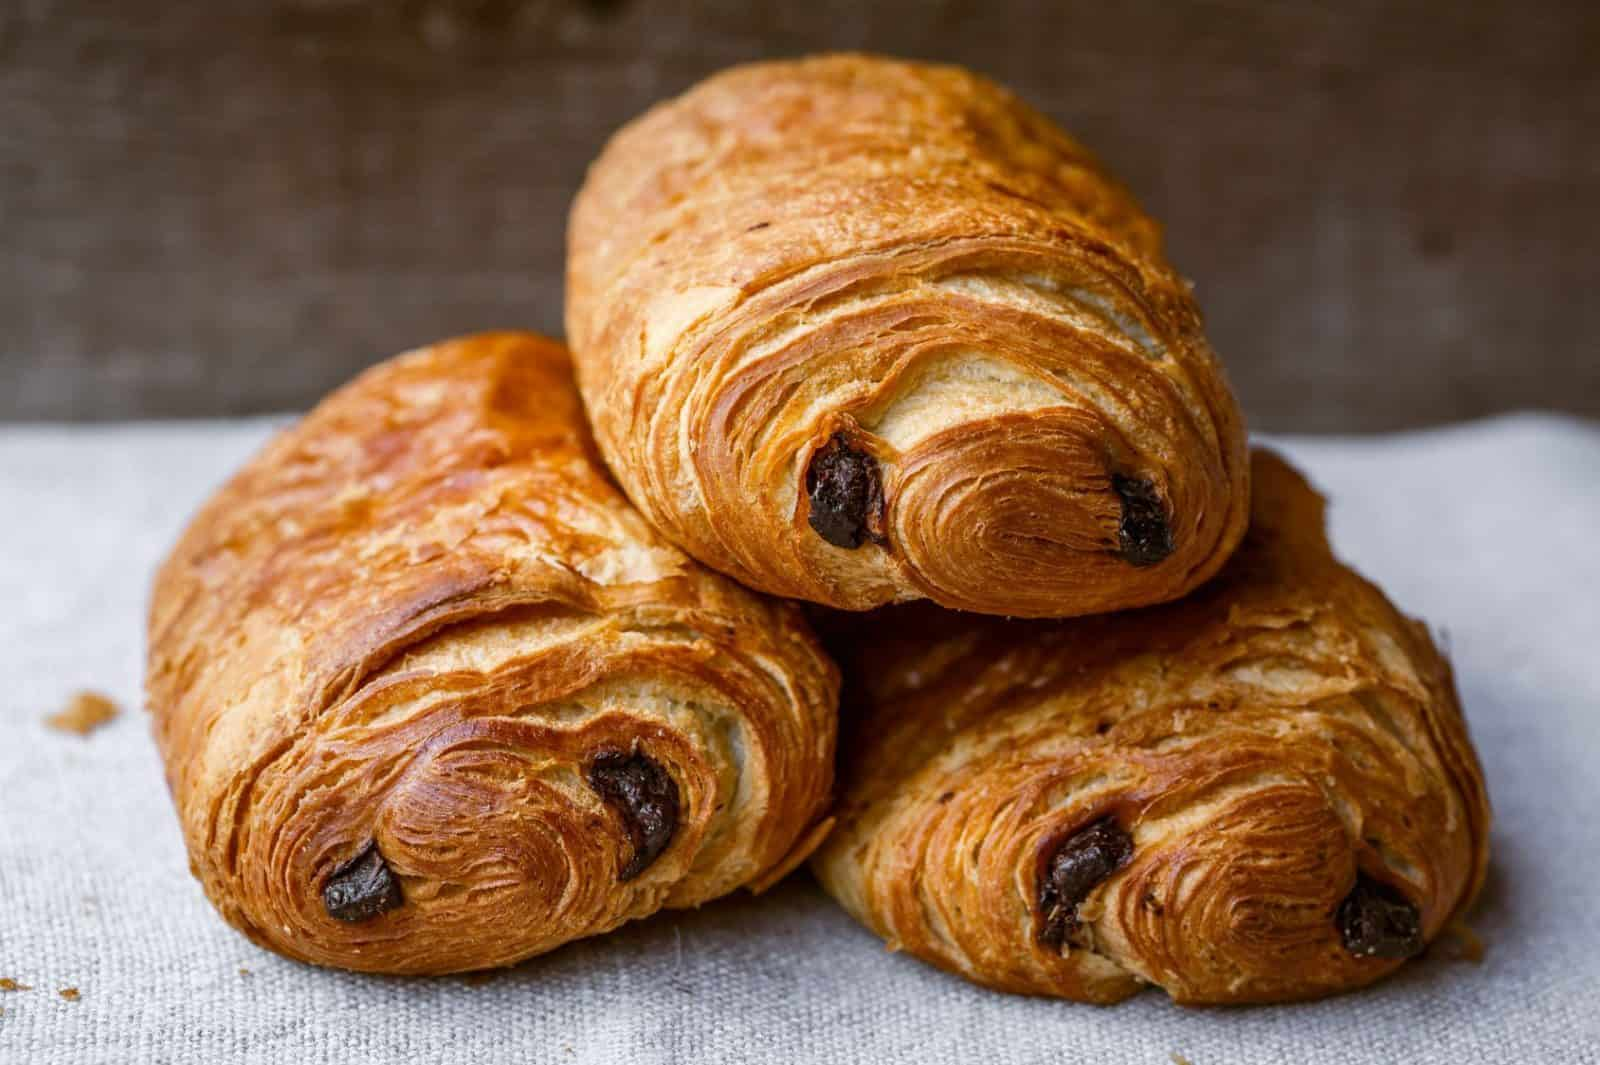
\includegraphics[scale=0.07]{pain_chocolat.jpg} \\
              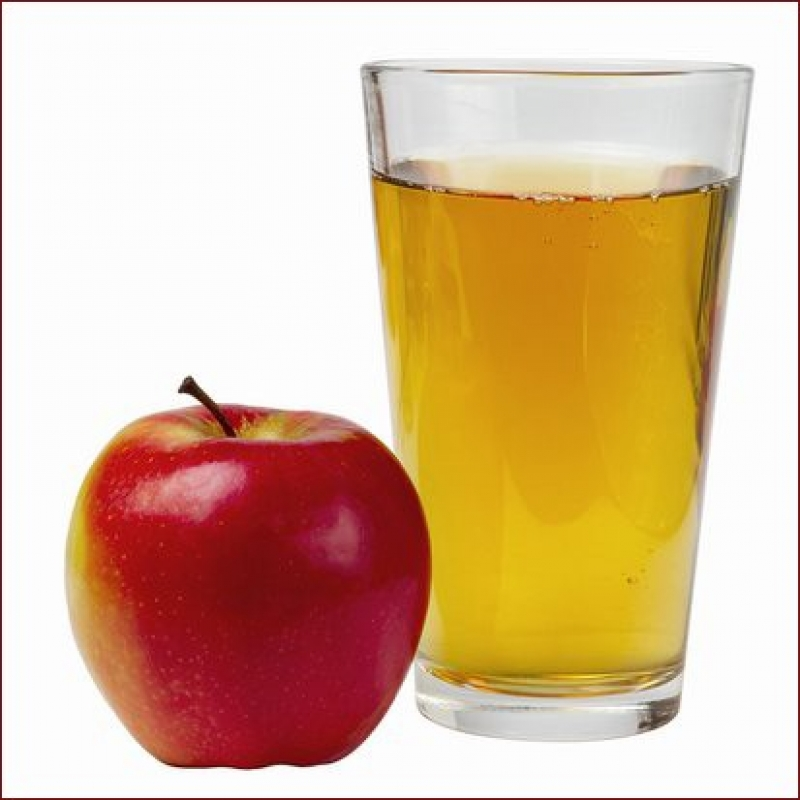
\includegraphics[scale=0.15]{jus_pomme.jpg}
            }
            \only<7-9>{
              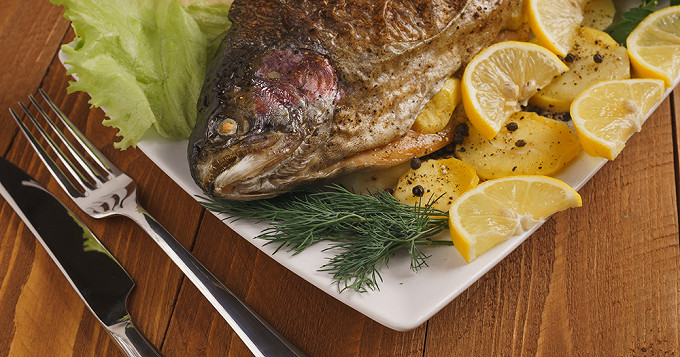
\includegraphics[scale=0.25]{poisson.jpeg} \\
              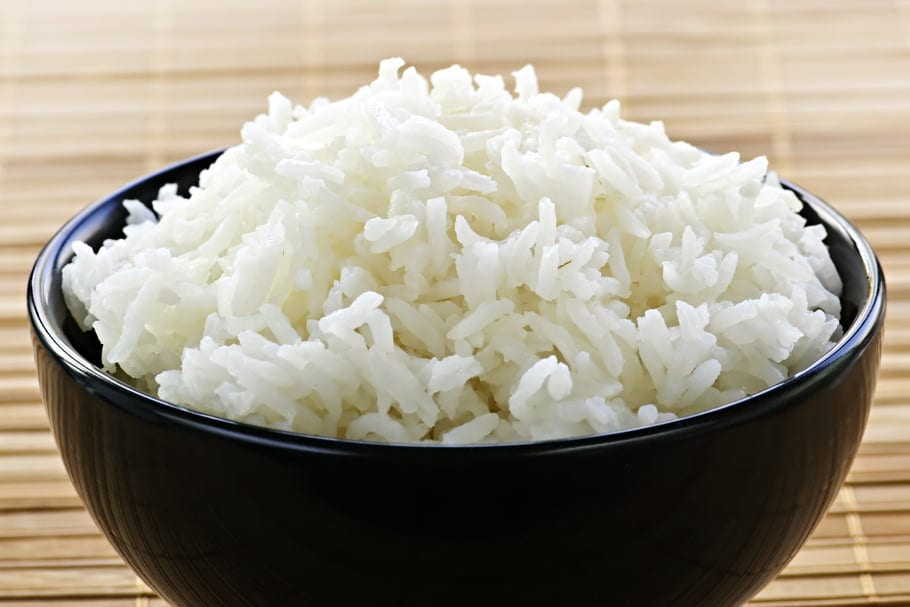
\includegraphics[scale=0.125]{riz.jpg}
            }
            \only<10-12>{
              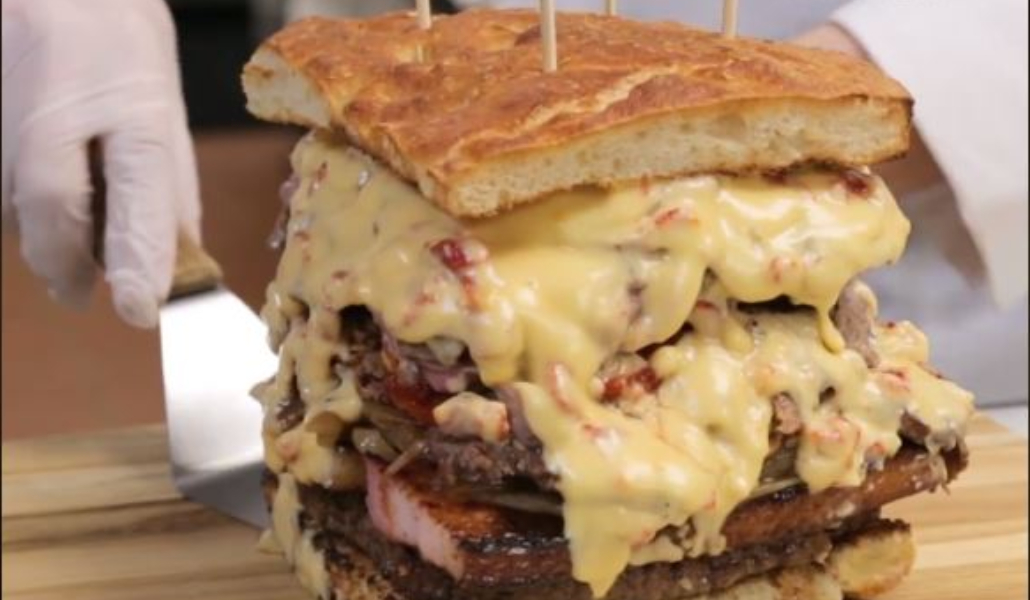
\includegraphics[scale=0.125]{sandwich.jpg} \\
              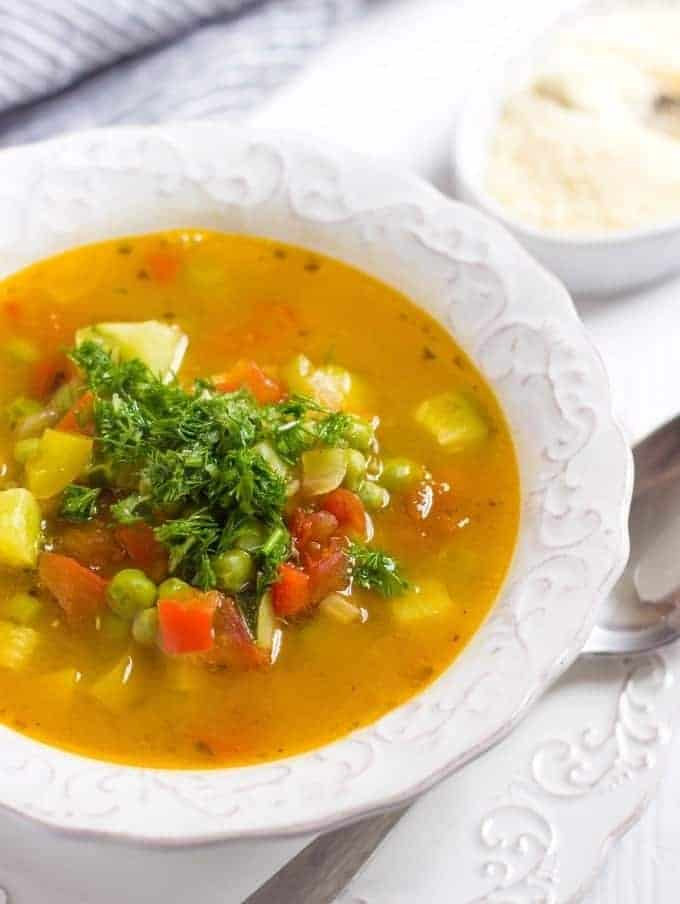
\includegraphics[scale=0.12]{soupe.jpg}
            }
            \only<13-15>{
              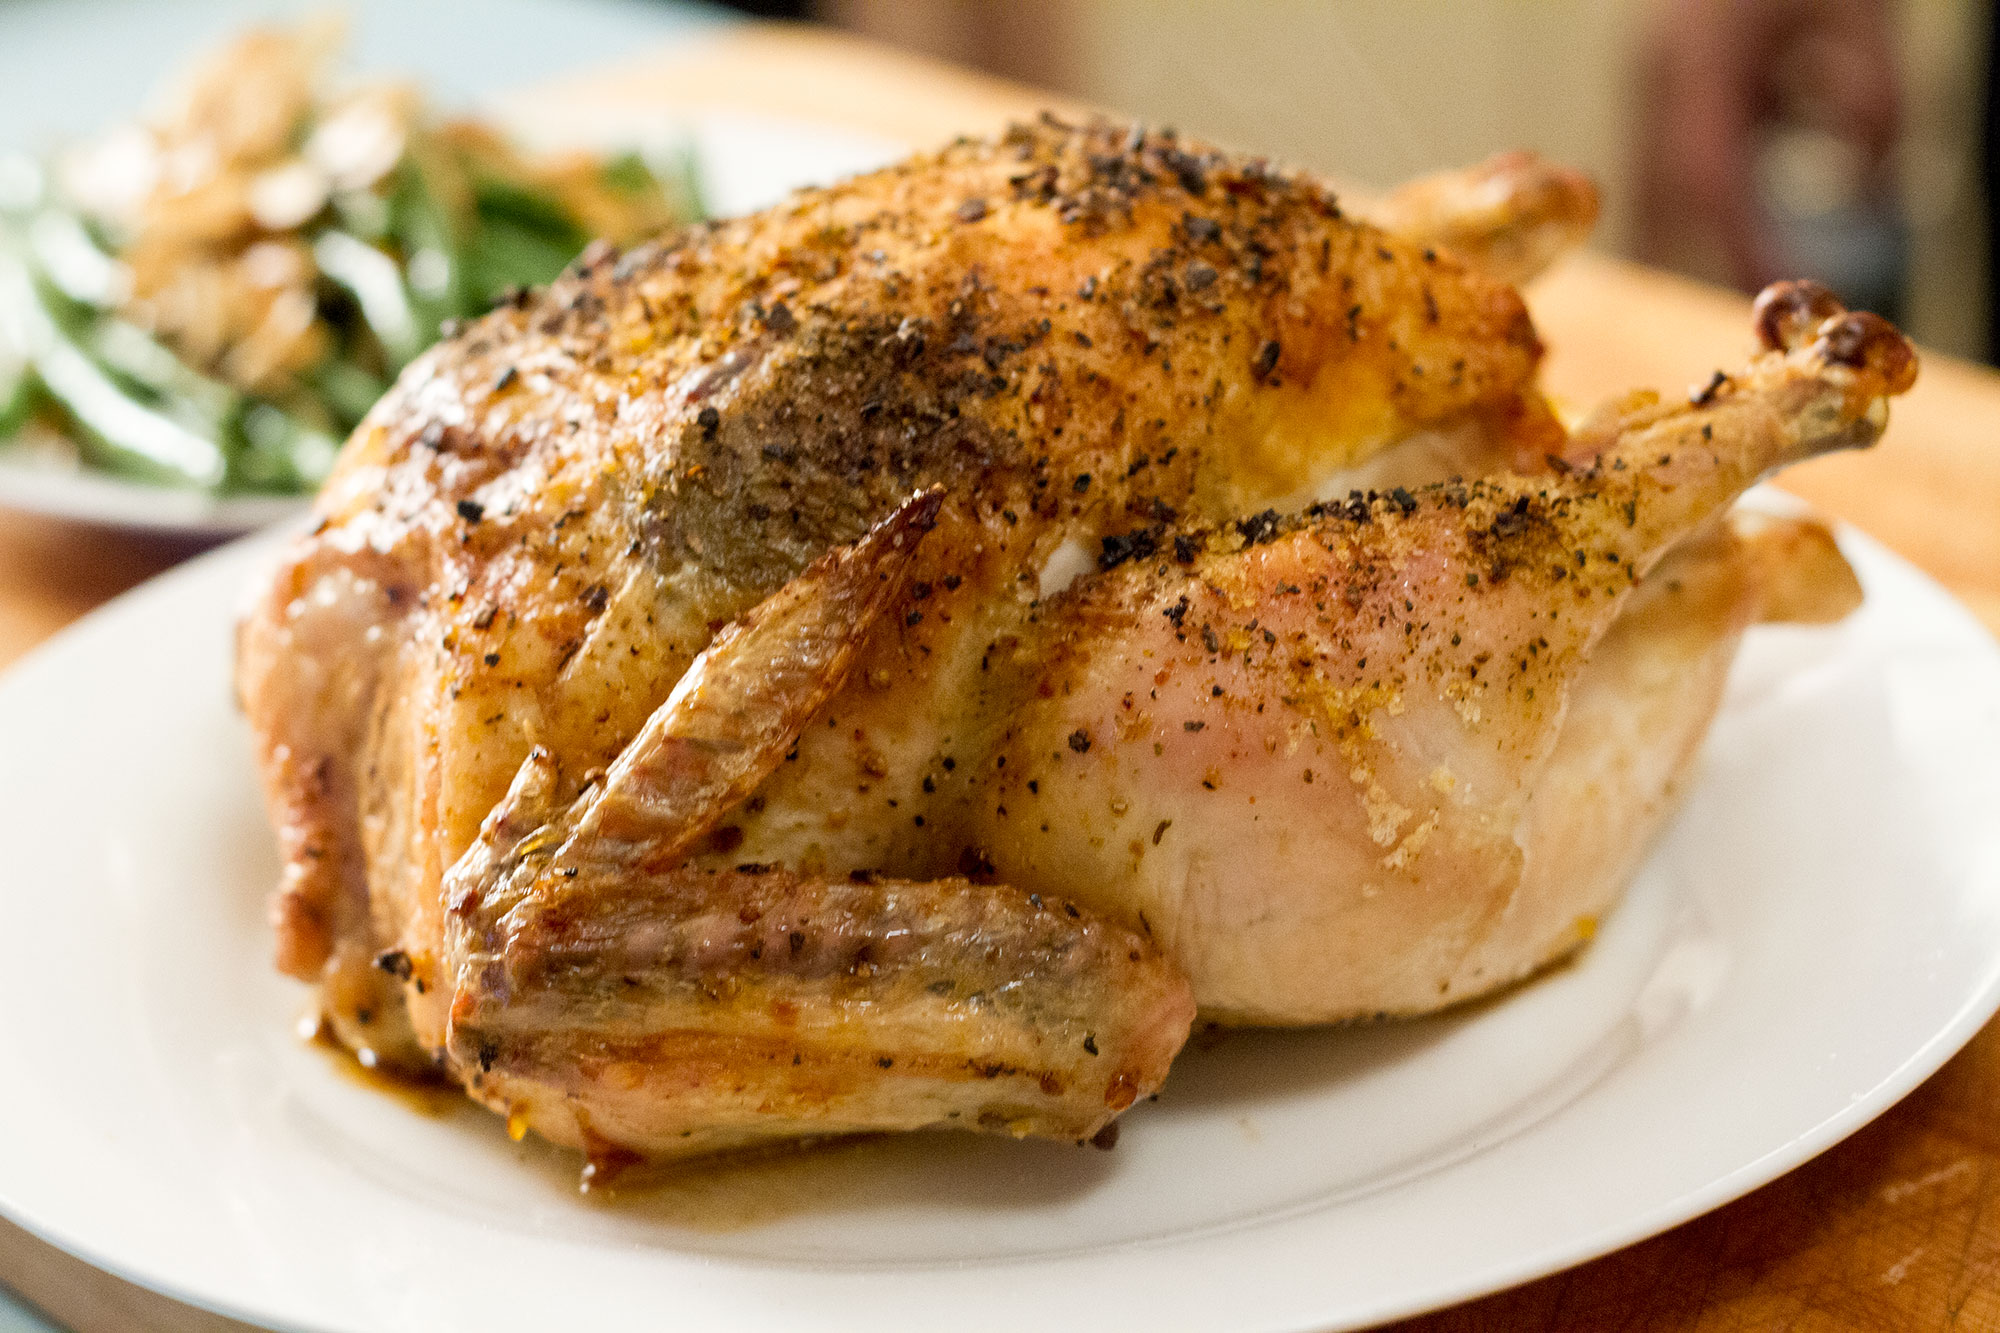
\includegraphics[scale=0.07]{poulet.jpg} \\
              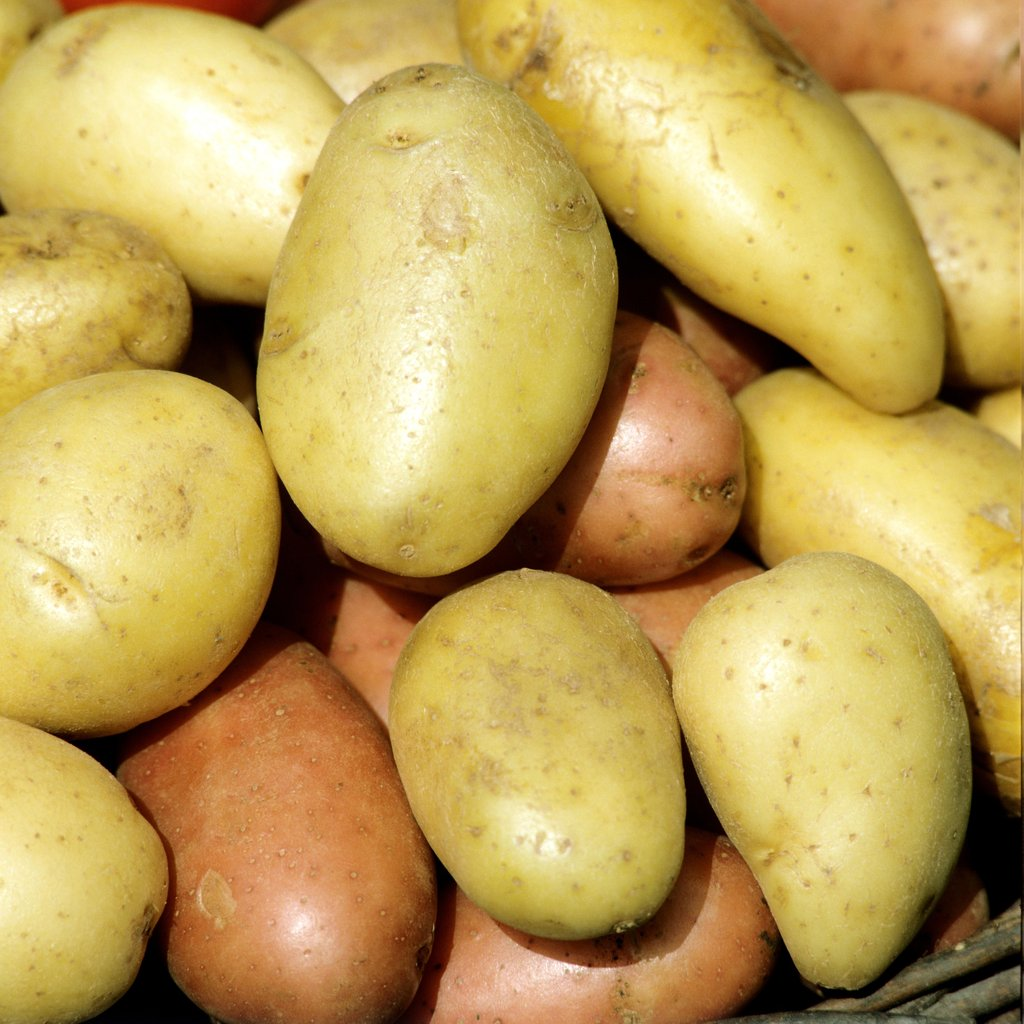
\includegraphics[scale=0.18]{patates.jpg}
            }
          \end{center}
        \end{minipage}
    \end{columns}
  \end{frame}

  \begin{frame}{}
    \begin{center}
      \Large Quiz
    \end{center}
  \end{frame}

  \begin{frame}{Je mets et je jette...}
    Avec un/e partenaire, discuter quels aliments tu \alert{mets} sur les plats suivants et quels aliments tu \alert{jettes}. \\
    \tinygloss{With a partner, discuss which foods you \alert{put} on the following dishes and which foods you \alert{throw away} (i.e., don't put on).}
    \begin{description}
      \item[] \textbf{Modèle:} \emph{une quiche}
      \item[E1:] Moi, je mets du fromage, des œufs et du beurre, mais je jette du bacon et du poulet.
    \end{description}
    \begin{columns}
      \column{0.5\textwidth}
        \begin{enumerate}
          \item une salade composée
          \item un sandwich
          \item une salade de fruits
          \item une tranche de pain grillé
          \item un café
        \end{enumerate}
      \column{0.5\textwidth}
        \begin{enumerate}
          \setcounter{enumi}{5}
          \item des frites
          \item un poulet
          \item une pomme de terre
          \item une pizza
          \item un yaourt
        \end{enumerate}
    \end{columns}
  \end{frame}

  \begin{frame}{Mais pourquoi?}
    Demande à un/e partenaire pourquoi il/elle fait les choses suivantes. \\
    \tinygloss{Ask a partner why they do the following things.}
    \begin{description}
      \item[] \textbf{Modèle:} \emph{ne pas appeler tes parents}
      \item[E1:] Pourquoi est-ce que tu n'appelles pas tes parents?
      \item[E2:] Je n'aime pas parler au téléphone.
    \end{description}
    \begin{columns}[t]
      \column{0.5\textwidth}
        \begin{enumerate}
          \item acheter beaucoup de biscuits
          \item jeter les bouteilles vides \gloss{empty}
          \item ne pas te lever avant midi
          \item ne pas épeler correctement mon nom
        \end{enumerate}
      \column{0.5\textwidth}
        \begin{enumerate}
          \setcounter{enumi}{4}
          \item acheter toujours des chips et du chocolat
          \item appeler tous tes amis avec mon portable
          \item jeter les tomates
        \end{enumerate}
    \end{columns}
  \end{frame}

  \begin{frame}{}
    \begin{center}
      \Large Questions?
    \end{center}
  \end{frame}
\end{document}
